\documentclass[12pt]{article}
%\usepackage{ucs}
\usepackage{amsmath,amssymb,amsthm}
%\usepackage{pb-diagram}
\usepackage{multicol}
\usepackage{cmap}
\usepackage{color}
\usepackage{graphicx}
\usepackage{epstopdf}
\usepackage{hyperref}

%\usepackage{verbatim}
%\newenvironment{comment}
%{\par\noindent{\bf TODO}\\}
%{\\\hfill$\scriptstyle\blacksquare$\par}

\newtheorem{statement}{Statement}
\newtheorem{theorem}{Theorem}
\newtheorem{corollary}{Corollary}[theorem]
\newtheorem{lemma}{Lemma}
\newtheorem{mynote}{Note}[section]
\theoremstyle{definition}
\newtheorem{definition}{Definition}
\newtheorem{remark}{Remark}
\newcommand{\go}{\stackrel{\circ }{\mathfrak{g}}}
\newcommand{\ao}{\stackrel{\circ }{\mathfrak{a}}}
\newcommand{\co}[1]{\stackrel{\circ }{#1}}
\newcommand{\pia}{\pi_{\mathfrak{a}}}
\newcommand{\piab}{\pi_{\mathfrak{a}_{\bot}}}

\newcommand{\gf}{\mathfrak{g}}
\newcommand{\af}{\mathfrak{a}}
\newcommand{\afb}{\mathfrak{a}_{\bot}}
\newcommand{\hf}{\mathfrak{h}}
\newcommand{\hfb}{\mathfrak{h}_{\bot}}
\newcommand{\pf}{\mathfrak{p}}

\begin{document}
\title{Nope}
\author{V D Lyakhovsky$^1$ and A A Nazarov$^2$}
%\address{$^{1,2}$ Theoretical Department, SPb State University,
%198904, Sankt-Petersburg, Russia }
%\eads{$^1$ \mailto{lyakh1507@nm.ru}, $^2$ \mailto{antonnaz@gmail.com}}

\begin{abstract}
\end{abstract}

\section{Introduction}
\label{sec:introduction}

We consider the reduction problem for simple Lie algebra modules. We study the reduction of Verma and irreducible finite-dimensional modules of the algebra to the modules of the subalgebra. We discuss the connection of the reduction with the Bernstein-Gelfand-Gelfand resolution. We show that different structures appear in the process of reduction, for example modules of contracted algebra and generalized Verma modules from parabolic category $\mathcal{O}^{\mathfrak{p}}$.

First of all, consider the following example. 
Let Lie algebra $\gf$ be $so(5)$ and subalgebra $\af\subset \gf$ be $so(3)$. There are different embeddings of $so(3)\to so(5)$. Here we limit ourselves to the regular ones. 
The root system of the algebra $so(5)$ consists of 8 roots. We denote simple roots by $\alpha_{1}=e_{1}-e_{2}$ and $\alpha_{2}=e_{2}$, where $e_{1},e_{2}$ form standard basis. The set of the positive roots is $\Delta^{+}=\left\{\alpha_{1}, \alpha_{1}+\alpha_{2}, \alpha_{1}+2\alpha_{2}, \alpha_{2}\right\}$. Each of these roots can be taken as the simple root of the subalgebra $so(3)$. At first we consider the subalgebra $so(3)$ with the root space spanned on $\beta=\alpha_{1}+2\alpha_{2}$. Verma module $M^{\mu}$ with the highest weight $\mu=\omega_{1}+2\omega_{2}=2\alpha_{1}+3\alpha_{2}$ is shown at Figure \ref{fig:B2_Verma}.
\begin{figure}[h!bt]
  \noindent\centering{
    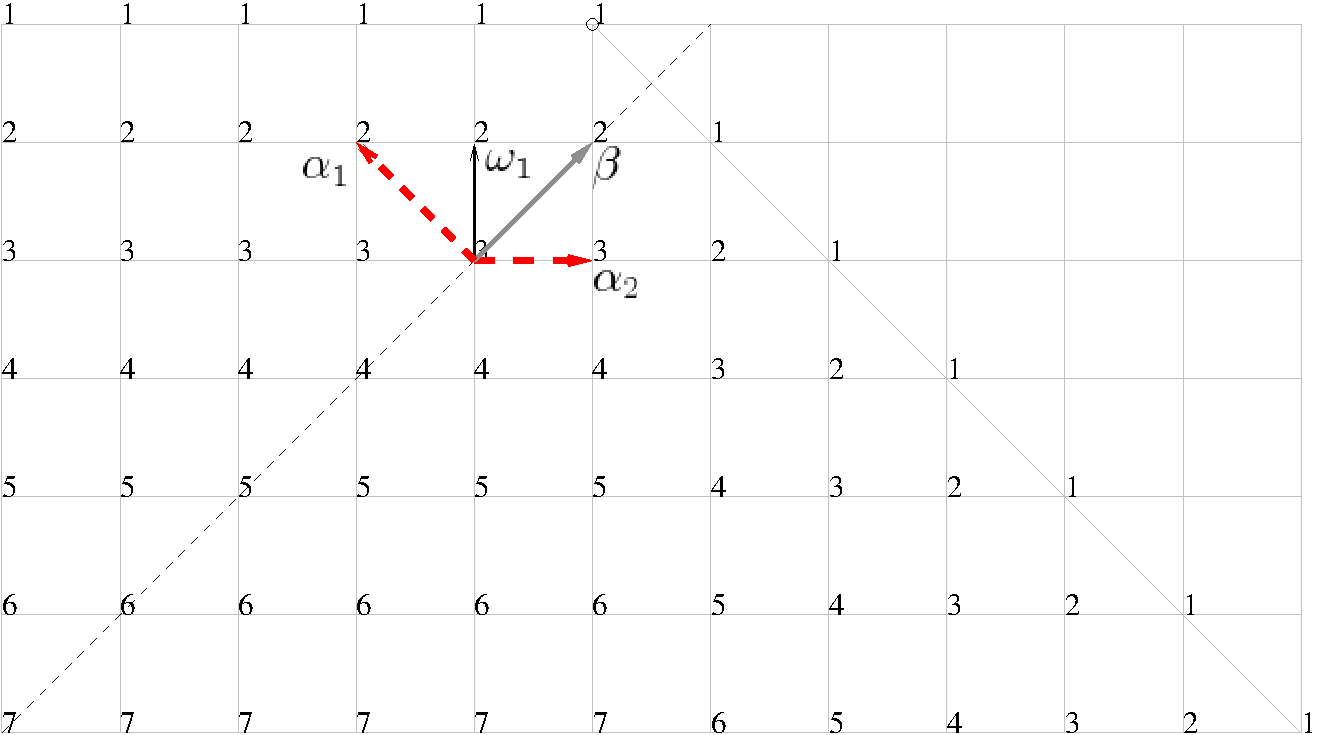
\includegraphics[width=120mm]{B2_Verma}
  }
  \caption{Regular embedding of $A_1$ into $B_2$. Simple roots $\alpha_1, \alpha_2$ of $B_2$ are presented as the dashed vectors.
    The simple root $\beta = \alpha_1+2\alpha_2$ of $A_1$ is indicated as the grey vector. Dimensions of weight subspaces of Verma module $M^{(1,2)}$ are shown.}
  
  \label{fig:B2_Verma}
\end{figure}

The branching coefficients are shown at Figure \ref{fig:B2_Verma_Branch2} for the different regular embeddings $so(3)\to so(5)$. Here we can see that the picture depends upon the embedding and looks similar to the Verma modules of some subalgebra.
\begin{figure}[h!bt]
  \noindent\centering{
    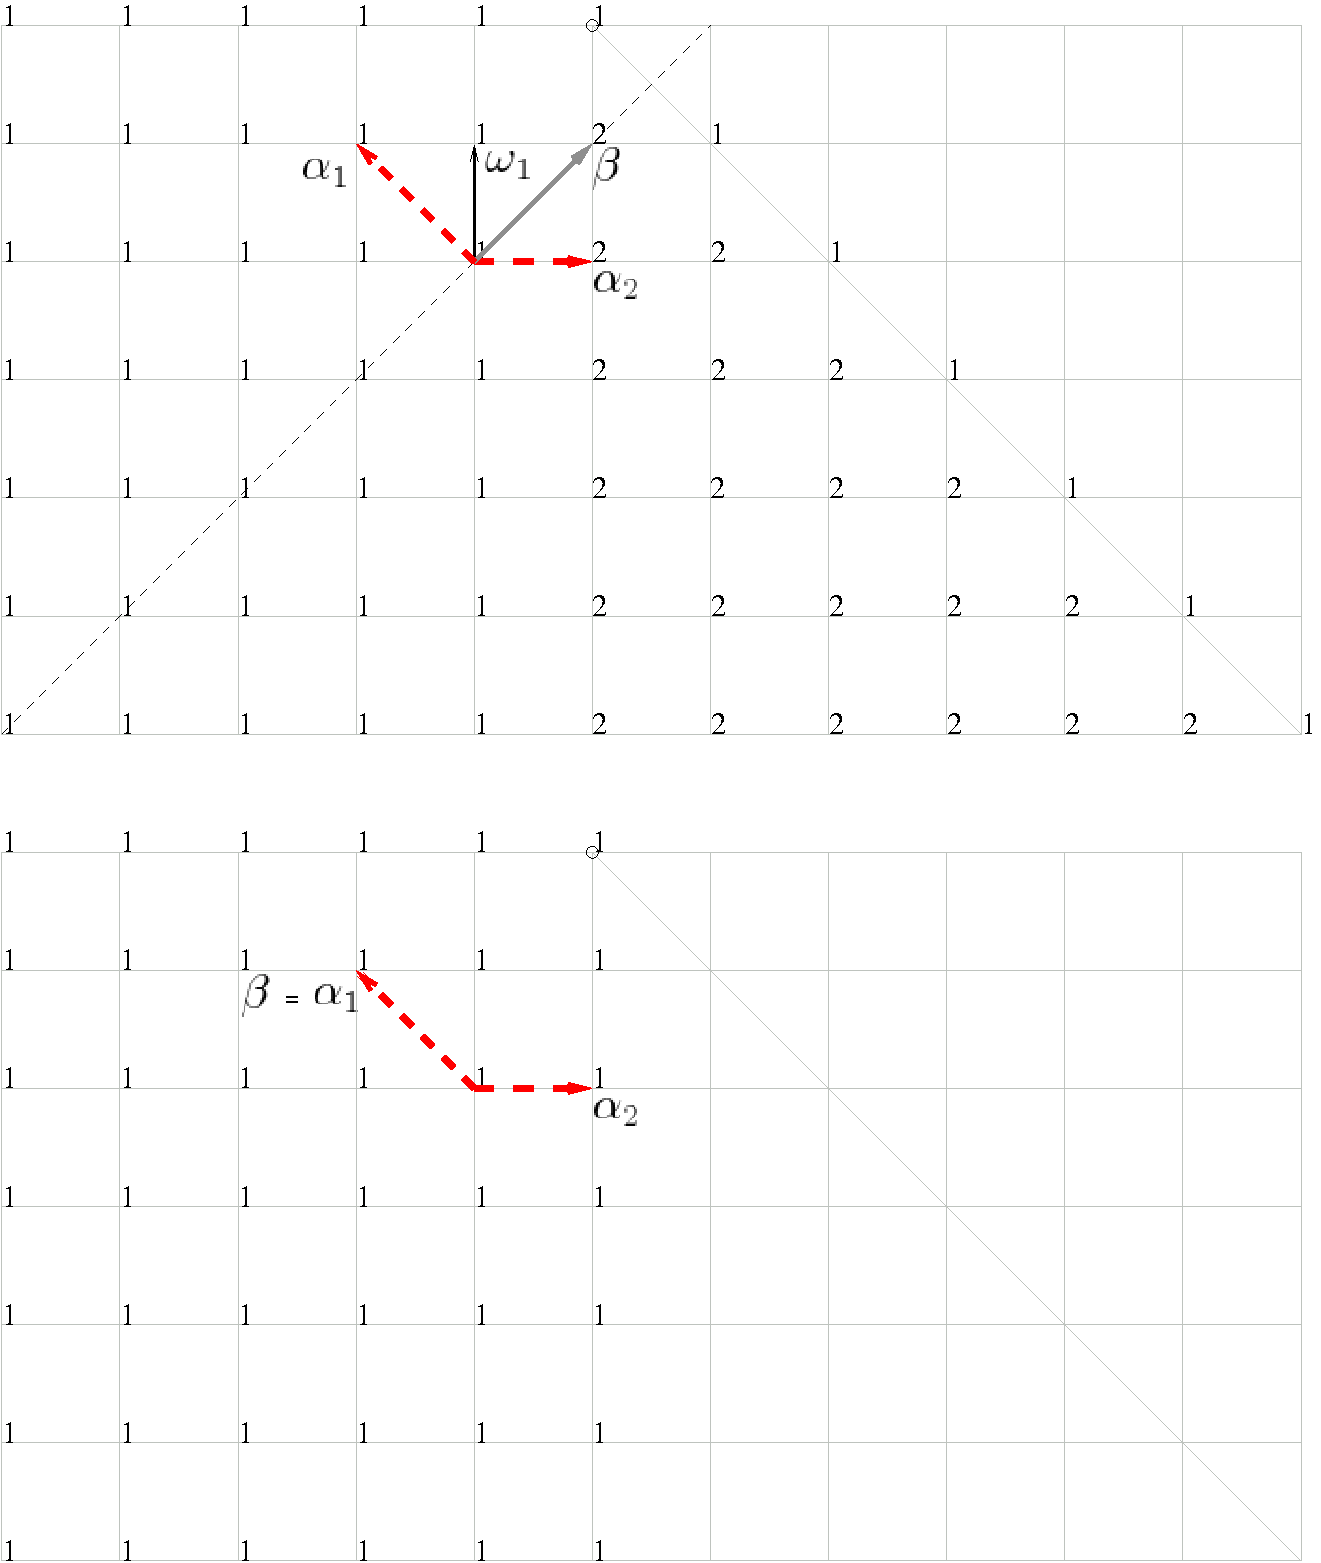
\includegraphics[width=120mm]{B2_Verma_Branch2}
  }
  \caption{Branching for the Verma modules}
  
  \label{fig:B2_Verma_Branch2}
\end{figure}
In present paper we interpret this branching coefficients as the dimensions of the weight subspaces of the modules of contracted algebras.


The formal character of Verma module is given by the expression
\begin{equation}
  \label{eq:17}
  \mathrm{ch} M^{\mu}=\frac{e^{\mu}}{\prod_{\alpha\in \Delta^{+}} \left(1-e^{-\alpha}\right)}
\end{equation}
The denominator $R=\prod_{\alpha\in \Delta^{+}} \left(1-e^{-\alpha}\right)$ can be rewritten as the sum over the Weyl group of the algebra
\begin{equation}
  \label{eq:20}
  R=\sum_{w\in W} \epsilon(w) e^{w\rho-\rho}.
\end{equation}
Since we consider the regular embeddings, all the positive roots of the subalgebra $\af$ are in the set of positive roots of the algebra $\gf$, $\Delta^{+}_{\af}\subset \Delta^{+}$. Then we can introduce $\tilde R$ and the carrier of its expansion $\Phi$:
\begin{equation}
  \label{eq:21}
  \tilde R=\prod_{\alpha\in \Delta^{+}\setminus \Delta^{+}_{\af}} \left( 1 - e^{-\alpha}\right)=-\sum_{\gamma\in \Phi} s(\gamma) e^{-\gamma}
\end{equation}
The ordering of roots in $\Delta _{\af}$ induce the
natural ordering of the weights in $P_{\af}$. Denote by $\gamma _{0}$
the lowest vector of $\Phi _{\af\subset \frak{g}}$ . The set
\begin{equation}
\Gamma _{\af\rightarrow \frak{g}}=\left\{ \xi -\gamma _{0}|\xi \in \Phi _{%
\af\subset \frak{g}}\right\} \setminus \left\{ 0\right\}
\label{fan-defined}
\end{equation}
is called the \textit{injection fan}.


The root of the subalgebra is among the positive roots of the algebra. So  Verma module can be decomposed into the set of Verma modules of the subalgebra:
\begin{equation}
  \label{eq:18}
  \mathrm{ch}M^{\mu}=\sum_{\nu}b^{(\mu)}_{\nu} e^{\nu-\pi_{\af}\nu} \mathrm{ch}M^{\pi_{\af}\nu}_{\af}
\end{equation}
Using the equation \eqref{eq:21} we can write the recurrent relation for the branching coefficients $b^{(\mu)}_{\nu}$:
\begin{equation}
  \label{eq:19}
   b_{\xi }^{\left( \mu \right) }=-\frac{1}{s\left( \gamma _{0}\right) }\left(
        \delta_{\xi-\gamma_0,\mu}
        +\sum_{\gamma \in
          \Gamma _{\af \rightarrow \gf}}s\left( \gamma +\gamma _{0}\right) b_{\xi
          +\gamma }^{\left( \mu \right) }\right).
\end{equation}

\section{Regular subalgebras and generalized Verma modules}
\label{sec:regul-subalg-gener}

Consider finite-dimensional Lie algebra $\mathfrak{g}$  and its regular reductive subalgebra $\af\subset \mathfrak{g}$. Introduce the following objects.
\begin{definition}
  \label{def-1}
  Denote by $\Delta^{+}_{\afb}=\left\{\alpha\in \Delta^{+}_{\mathfrak{g}}:\forall \beta\in\Delta_{\af} \; \alpha\bot \beta\right\}$ the subset of the positive roots of $\mathfrak{g}$ orthogonal to the root system of $\af$.
\end{definition}

\begin{definition}
  \label{def-2}
  Denote by $W_{\afb}$ the subgroup of the Weyl group $W$ generated by the reflections $w_{\alpha}$ corresponding to the roots $\alpha\in \Delta^{+}_{\afb}$.
\end{definition}
\begin{mynote}
  The subgroup $W_{\afb}$ preserves $\Delta_{\af}$ since it is generated by the reflections in hyperplanes containing $\Delta_{\af}$.
\end{mynote}
\begin{definition}
  \label{def-3}
  The subsystem $\Delta_{\afb}=\Delta^{+}_{\afb}\cup \left(-\delta^{+}_{\afb}\right)$ determines the subalgebra $\af_{\bot}\subset \mathfrak{g}$.
\end{definition}
Let
\begin{equation*}
\frak{h}_{\perp }^{\ast }:=\left\{ \eta \in \frak{h}_{\perp \af}^{\ast
}|\forall \alpha \in \Delta _{\af}\cup \Delta _{\af_{\perp
}};\alpha \bot \eta \right\}
\end{equation*}
and consider the subalgebras
\begin{eqnarray*}
\widetilde{\af_{\perp }} &:&=\af_{\perp }\oplus \frak{h}_{\perp }
\\
\widetilde{\af} &:&=\af\oplus \frak{h}_{\perp }.
\end{eqnarray*}
Algebras $\af$ and $\af_{\perp }$ form the ''orthogonal pair''
$\left( \af,\af_{\perp}\right) $
of subalgebras in $\frak{g}$.

For the Cartan subalgebras we have the decomposition
\begin{equation}
\frak{h}=\frak{\frak{h}_{\af}}\oplus \frak{h}_{\af_{\perp }}\oplus
\frak{h}_{\perp }=\frak{\frak{h}_{\widetilde{\af}}}\oplus \frak{h}_{%
\af_{\perp }}=\frak{\frak{h}_{\widetilde{\af_{\perp }}}}\oplus
\frak{h}_{\af}.
\end{equation}
For the subalgebras of an orthogonal pair $\left( \af,\af_{\perp
}\right) $ we consider the corresponding Weyl vectors, $\rho _{\af}$
and $\rho _{\af_{\perp }}$ , and\ form the so called ''defects'' $%
\mathcal{D}_{\af}$ and $\mathcal{D}_{\af_{\perp }}$ of the
injection:
\begin{equation}
\mathcal{D}_{\af}:=\rho _{\af}-\pi _{\af}\rho ,
\end{equation}
\begin{equation}
\label{defect-perp}
\mathcal{D}_{\af_{\perp }}:=\rho _{\af_{\perp }}-\pi _{\af%
_{\perp }}\circ\rho .
\end{equation}
\begin{equation}
U:=\left\{ u\in W|\quad \mu _{\widetilde{\af_{\perp }}}\left( u\right)
\in \overline{C_{\widetilde{\af_{\perp }}}}\right\} \quad .
\label{U-def}
\end{equation}
For the same set $U$ introduce the weights
\begin{equation*}
\mu _{\af}\left( u\right) :=\pi _{\af}\circ\left[ u(\mu +\rho )-\rho %
\right] +\mathcal{D}_{\af_{\perp }}.
\end{equation*}
To simplify the form of relations we shall now on omit the sign "$\circ$" in projected
weights.

Let us state the following lemma.
\begin{lemma}
\label{lemma-1}
The quotient of the singular weights element $\Psi^{(\mu)}$ by the denominator $R_{\af_{\bot}}$ is given by the formal element corresponding to the modified set of the singular weights of $L_{\af\oplus\mathfrak{h}_d}^{(\pi_{\af\oplus\mathfrak{h}_d}\mu)}$ with the multiplicities given by the dimensions of $\af_{\bot}$-modules.
\begin{equation}
  \label{eq:4}
  \frac{\Psi^{(\mu)}_{\mathfrak{g}}}{\prod_{\alpha\in \Delta^{+}_{\afb}}\left(1-e^{-\alpha}\right)^{\mathrm{mult}(\alpha)}}=
    \sum_{u\in W/W_{\afb}}\epsilon(u)e^{\pi_{\tilde\af}\left[(u(\mu+\rho)-\rho)\right]+\mathcal{D}}\cdot \mathrm{ch}_{\af_{\bot}}
      L^{\piab(u(\mu+\rho)-\rho)-\mathcal{D}}
\end{equation}
\end{lemma}  
\begin{proof}
  Consider $\Psi^{(\mu)}_{\mathfrak{g}}$. It is given by the sum over the Weyl group.
  \begin{equation}
    \label{eq:6}
    \Psi^{(\mu)}_{\mathfrak{g}}=\sum_{w\in W}\epsilon(w)e^{w(\mu+\rho)-\rho}
  \end{equation}
  We can divide the summation to the sum over $W_{\afb}$ and sum over all the classes of $W/W_{\afb}$: $w=vu,\; v\in W_{\afb},\; u \in W/W_{\afb}$. We have the following obvious property of the projections:
  \begin{equation}
    \label{eq:5}
    u(\mu+\rho)=\pia(u(\mu+\rho))+\piab(u(\mu+\rho))+\pi_{h_{\perp}^*}(u(\mu+\rho))
  \end{equation}
 Since $\mathfrak{h}_{\af}^*,\mathfrak{h}_{\perp}^*$ are invariant under the action of $v\in W_{\afb}$, we have
  \begin{equation}
    \label{eq:8}
    vu(\mu+\rho)-\rho=v\cdot(\piab(u(\mu+\rho))-\rho_{\afb}+\rho_{\afb})-\rho_{\afb}+\pia(u(\mu+\rho))-\rho+\rho_{\afb}+\pi_{\hf_{\perp}^*}(u(\mu+\rho))
  \end{equation}
  Only the first term depends on $v$. So
  \begin{equation}
    \label{eq:9}
    \frac{\Psi^{(\mu)}_{\mathfrak{g}}}{\mathrm{R}_{\afb}}=
    \frac{\sum_{u\in W/W_{\afb}}\epsilon(u)e^{\pia(u(\mu+\rho))-\rho+\rho_{\afb}+\pi_{\mathfrak{h}_{\perp}}(u(\mu+\rho))}\cdot
      \sum_{v\in W_{\afb}}\epsilon(v)e^{v(\piab u(\mu+\rho)-\rho_{\afb}+\rho_{\afb})-\rho_{\afb}}}{\mathrm{R}_{\afb}}
  \end{equation}
  We can rewrite the r.h.s. as
  \begin{equation}
    \label{eq:10}
    \sum_{u\in W/W_{\afb}}\epsilon(u)e^{\pi_{(\af\oplus\mathfrak{h}_d)}\left[u(\mu+\rho)-\rho\right]+\pi_{(\af\oplus \mathfrak{h}_d)}\cdot \rho-\rho+\rho_{\afb}}\cdot
    \mathrm{ch}_{\afb}L^{\pi_{\afb}u(\mu+\rho)-\rho_{\afb}}.
  \end{equation}
  Since $\pi_{\afb}(u(\mu+\rho)-\rho)-(\rho_{\afb}-\pi_{\afb}\rho)=\pi_{\afb}(u(\mu+\rho)-\rho)-\mathcal{D}$ and $\pi_{\tilde\af}\rho-\rho=-\pi_{\afb}\rho$ we get the statement of the Lemma.

\end{proof}

\begin{corollary}
  \label{sec:corollary-1}
  If we apply the projection $\pi_{\af}$ to the subalgebra $\af$ to the equation (\ref{eq:4}) we obtain the ``Lemma 1'' from the paper \cite{2010arXiv1007.0318L} in the case of regular subalgebras $\af, \afb$. However this Lemma \ref{lemma-2} is more general then Lemma \ref{lemma-1}, since it holds for the special subalgebra $\af$.
\begin{lemma}
\label{lemma-2}
Let $\af$ and $\af_{\perp }$ be the orthogonal pair of regular
subalgebras in $\frak{g}$, with $\widetilde{\af_{\perp }}=\af%
_{\perp }\oplus \frak{h}_{\perp }$ and $\widetilde{\af}=\af\oplus
\frak{h}_{\perp }$ ,

$L_{\frak{g}}^{\mu }$ be the highest weight module with the singular element
$\Psi _{\frak{g}}^{\mu }$ ,

$R_{\af_{\perp }}$ be the Weyl denominator for $\af_{\perp }$.

Then the element $\pi _{\af}\left( \frac{\Psi _{\frak{g}}^{\mu }}{R_{%
\af_{\perp }}}\right) $ can be decomposed into the sum over $u\in U$ (see (\ref{U-def})) of
the singular elements $e^{\mu _{\af}\left( u\right) }$ with the
coefficients $\epsilon (u)\mathrm{\dim }\left( L_{\widetilde{\af_{\perp
}}}^{\mu _{\widetilde{\af_{\perp }}}\left( u\right) }\right) $:
\begin{equation}
\quad \pi _{\af}\left( \frac{\Psi _{\frak{g}}^{\mu }}{R_{\af%
_{\perp }}}\right) =\sum_{u\in U}\;\epsilon (u)e^{\mu _{\af}\left(
u\right) }\mathrm{\dim }\left( L_{\widetilde{\af_{\perp }}}^{\mu _{%
\widetilde{\af_{\perp }}}\left( u\right) }\right) .
\label{eq:11}
\end{equation}
\end{lemma}
This lemma can be used to state the recurrent relation for the branching coefficients for the reduction of $\gf$-module to $\af$-modules. (See \cite{2010arXiv1007.0318L} for the details). It will be also useful for the discussion of special subalgebras. 
\end{corollary}
\begin{corollary}
  \label{corollary-2}
  Since $\af, \afb$ are regular subalgebras the simple root system $\alpha_1,\dots, \alpha_r$ of $\gf$ can be chosen in such a way that simple roots $\beta_1,\dots,\beta_{r_{\afb}}$ of $\afb$ are contained in it. Denote the set of roots $\beta_i$ by $I$. This notation is in the agreement with the book \cite{humphreys2008representations}.
  \begin{equation*}
    I=\{\beta_1,\dots,\beta_{r_{\afb}}\}\subset \{\alpha_1,\dots,\alpha_r\}
  \end{equation*}
  Then the subset $I$ determines not only the subalgebra $\afb$, but also the minimal parabolic subalgebra $\mathfrak{p}_I$, such that $\afb\subset \mathfrak{p}$. Then we can consider the modules of the subcategory $\mathcal{O}^{\mathfrak{p}}$, for example the generalized Verma modules $M_{\mathfrak{p}}^{(\mu)}$. This modules are constructed from the irreducible highest-weight modules $L_{\pf}^{(\mu)}$ as follows
  \begin{equation}
    \label{eq:1}
    M_{\pf}^{(\mu)}=U(\gf)\otimes_{U(\pf)} L^{(\mu)}_{\pf}
  \end{equation}
  Denote by $\tilde R$ the denominator constructed of the positive roots of $\gf$ which are not the roots of $\afb$.
  \begin{equation}
    \label{eq:2}
    \tilde R = \prod_{\alpha\in \Delta^+\setminus \Delta^{+}_{\afb}} \left(1-e^{-\alpha}\right)^{\mathrm{mult}_{\gf} \alpha}
  \end{equation}
If we expand $\frac{1}{\tilde R}$ the coefficients near the terms $e^{\xi}$ are given by the Kostant partition function $p^I$ constructed from the roots of $\gf$ which are not in $I$. 
The character of the generalized Verma module then can be formally written as
\begin{equation}
  \label{eq:3}
  \mathrm{ch} M^{(\mu)}_{\pf}=\frac{1}{\tilde R} \mathrm{ch}L^{(\mu)}_{\pf}
\end{equation}
The character of the irreducible finite-dimensional $\pf$-module $L^{(\mu)}_{\pf}$ differs from the character of the irreducible finite-dimensional $\afb$-module by the factor $e^{\pi_{\tilde\af}(\mu)}$, since $\pf$ contains the full Cartan subalgebra $\hf\subset\gf$.
Now if we multiply the statement (\ref{eq:4}) of the lemma \ref{lemma-1} by $\frac{1}{\tilde R}$ we get the character of irreducible highest-weight module $L^{(\mu)}$ on the left and the sum of the characters of generalized Verma modules on the right-hand side of the equation:
\begin{multline}
  \label{eq:7}
  \mathrm{ch}L^{(\mu)}_{\gf}=
  \sum_{u\in W/W_{\afb}}\epsilon(u)e^{\pi_{\af\oplus\mathfrak{h}_d}\left[(u(\mu+\rho)-\rho)\right]+\mathcal{D}}\cdot \frac{1}{\tilde R}\mathrm{ch} L_{\afb}^{\piab(u(\mu+\rho)-\rho)-\mathcal{D}}=\\
  \sum_{u \in W/W_{\afb}} \epsilon(u) \mathrm{ch} M^{(u(\mu+\rho)-\rho)}_{\pf}
\end{multline}
So we have recovered the Bernstein-Gelfand-Gelfand resolution \cite{bernstein1975differential} for the parabolic category ${\cal O}^{\pf}$.
\end{corollary}

\section{Generalizations}
\label{sec:generalizations}

\begin{enumerate}
\item If $\af$ is a special subalgebra of $\gf$, the equation (\ref{eq:4}) and the Lemma \ref{lemma-1} no longer holds since the module of the algebra can not be presented as the composition of the modules of the subalgebra. Only the projection of this module can be decomposed. So we have to rely on the Lemma \ref{lemma-2}, which holds in this case too \cite{2010arXiv1007.0318L}.

Again as in the Corollary \ref{corollary-2} we can multiply the equation (\ref{eq:11}) by the (projection of) the denominator $\frac{1}{\tilde R}$. This projection if well-defined due to the construction of $\afb$.
\begin{equation}
  \label{eq:12}
  \pi_{\af}\left(\mathrm{ch} L^{(\mu)}_{\gf}\right)= \sum_{u\in U}\epsilon(u) \pi_{\af}\left(\frac{1}{\tilde R}\right) e^{\mu_{\af}(u)}\mathrm{dim} \left( L_{\widetilde{\af_{\perp }}}^{\mu _{%
\widetilde{\af_{\perp }}}\left( u\right) }\right) .
\end{equation}
Since the subalgebra $\afb$ is regular by construction,  at the right-hand side of the equation we see the generalized Verma module character projected on the root space of $\af$. So we have recovered the equation (\ref{eq:7}) in the projected form.
\begin{equation}
  \label{eq:13}
   \pi_{\af}\left(\mathrm{ch} L^{(\mu)}_{\gf}\right)= \pi_{\af}\left(  \sum_{u \in W/W_{\afb}} \epsilon(u) \mathrm{ch} M^{(u(\mu+\rho)-\rho)}_{\pf}\right)
\end{equation}
We have also lost any trace of subalgebra $\af$. But we can rewrite the left-hand side as the combination of the irreducible highest weight modules of subalgebra $\af$
\begin{equation}
  \label{eq:14}
  \sum_{\nu\in P^{+}_{\af}} b^{(\mu)}_{\nu} \mathrm{ch} L^{(\nu)}_{\af}= \sum_{u \in W/W_{\afb}} \epsilon(u) \pi_{\af}\left(   \mathrm{ch} M^{(u(\mu+\rho)-\rho)}_{\pf}\right)
\end{equation}
Using the Bernstein-Gelfand-Gelfand resolution for the subalgebra $\af$ we get the expression which links the projected characters of generalized Verma modules with the characters of Verma modules of special subalgebra:
\begin{equation}
  \label{eq:15}
  \sum_{\nu\in P^+_{\af}}b^{(\mu)}_{\nu}\sum_{ w\in W_{\af}} \epsilon(w) \mathrm{ch} M_{\af}^{w(\mu+\rho_{\af})-\rho_{\af}} =  \sum_{u \in W/W_{\afb}} \epsilon(u) \pi_{\af}\left(   \mathrm{ch} M^{(u(\mu+\rho)-\rho)}_{\pf}\right)
\end{equation}

\item Also we can generalize the whole construction to affine Lie algebras $\gf, \af$, since Weyl character formula and denominator identity have natural analogs in the theory of affine Lie algebras. The only subtle point is in the definition of projection $\pi$ to the subalgebra. The extension of the Killing form from the finite-dimensional simple Lie algebra $\co{\gf}$ to the affine Lie algebra $\gf$ is not positive-definite. For the imaginary root $\delta$ we have $(\delta,\delta)=0$. If we use this form for the projection to the root space of the affine subalgebra $\af$ we end up with $\delta\perp \beta; \beta\in \Delta_{\af}$ or $\pi_{\af}(n\delta)=0$. This is not what we want. 

So we define new positive-definite bilinear form $(\cdot,\cdot)_+$ on the root lattice of $\gf$ by the requirement $(\delta,\delta)_+=1$. This form is only $\co{W}$-invariant. Then we define the projection $\pi_{\af}$ to the root space of the affine subalgebra $\af$ as the extension of the projection to the finite-dimensional subalgebra $\co{\af}$ with the requirement
\begin{equation}
  \label{eq:16}
  \pi_{\af}(\delta)=\delta.
\end{equation}
The orthogonality conditions in the definitions \ref{def-1}, \ref{def-2}, \ref{def-3} are to be understood with the respect to the form $(\cdot,\cdot)_+$. Then Lemma \ref{lemma-1} holds for the affine Lie algebras $\gf, \af$.
\item Another case that we need to consider is the of $\afb$ built on the non-simple roots.
\end{enumerate}

\section{Applications}
\label{sec:applications}

\section{Conclusion}
\label{sec:conclusion}



\bibliography{article}{}
\bibliographystyle{utphys}

\end{document}
